\chapter{Introduction}

In this research, we explored various optimization techniques based on programming features for web servers. Initially, this research started with the idea of finding optimal web server architecture based on programming features of the Ballerina language. Several architectural changes were made to the original Ballerina server architecture. Thereafter, the performance of each server architecture is evaluated concerning different programs. Furthermore, server architectures were fine-tuned and it was able to identify that varying the thread pool size of the existing architecture is the best way to maximize the performance for a given set of programming features. Finally, a machine learning model was proposed to output the optimal thread pool size for a given set of programming features, and the model is evaluated with current Ballerina architecture.

\section{Background to the Research}

Web server optimization is a prominent branch in the enterprise-level software industry as well as e-businesses. Then services able to facilitate greater performance by consuming fewer computation resources. This research came along a long way from comparing the performance of different server architectures to thread pool optimization.  
Prior determination of web server architecture with the best performance is difficult due to various factors such as type of operations that execute (i.e IO and CPU intensive), workload, deployment environment, etc. Several studies have been conducted for both comparing the performance of server architectures and thread pool tuning. Pariag et al. \cite{comp_ac} have compared the performance of different server architectures under different workloads. Afterward, server architectures are extensively fine-tuned to optimize performance. Furthermore, the performance of architectures was maximized for workloads that perform IO operations. Several other studies have also discussed \cite{seda,events_are_bad,edprs} advantages and drawbacks of each severs architectures. Apart from that, several studies had pointed out that thread pool tuning was able to maximize the performance of web servers. Several mathematical models \cite{xu2004performance,thread_pool_analysis,math_aproach_thread_pool_tuning,syer2011identifying,linfeng2017design} and dynamic thread pool optimization techniques \cite{lorenzon2016investigating,nieplocha2007evaluating,agrawal2006adaptive} had been proposed in these studies. 

\newpage

\section{Research Problem and Research Questions}\label{sec:research_questions}
 
 In order to understand the following research questions, knowing the definition of web server architecture reffed in this study is important. It is explained in subsection \ref{sub:def_web_server_architecture}. This research addresses the following research questions,

\begin{itemize}
	
  	%\item What are the parameters required to tune in Ballerina's internal server architecture to maximize the performance for a given program type?
 	%\item Is it possible to propose optimal web server architecture or parameters based on program features?
 	
 	\item Is it possible to find a server architecture or parameters that would result in the best performance for a given Ballerina program? 
 	\item Is it possible to tune the thread pool size of a given server architecture in order to optimize the performance (i.e. throughput and latency)? If so what is the impact of the thread pool size on the performance for different Ballerina programs? 
 	\item Is it possible devise a model that can estimate the thread pool size that would result in the best performance for a given Ballerina program?
\end{itemize}


%%\begin{figure}[htbp]
%%  \begin{center}
%%    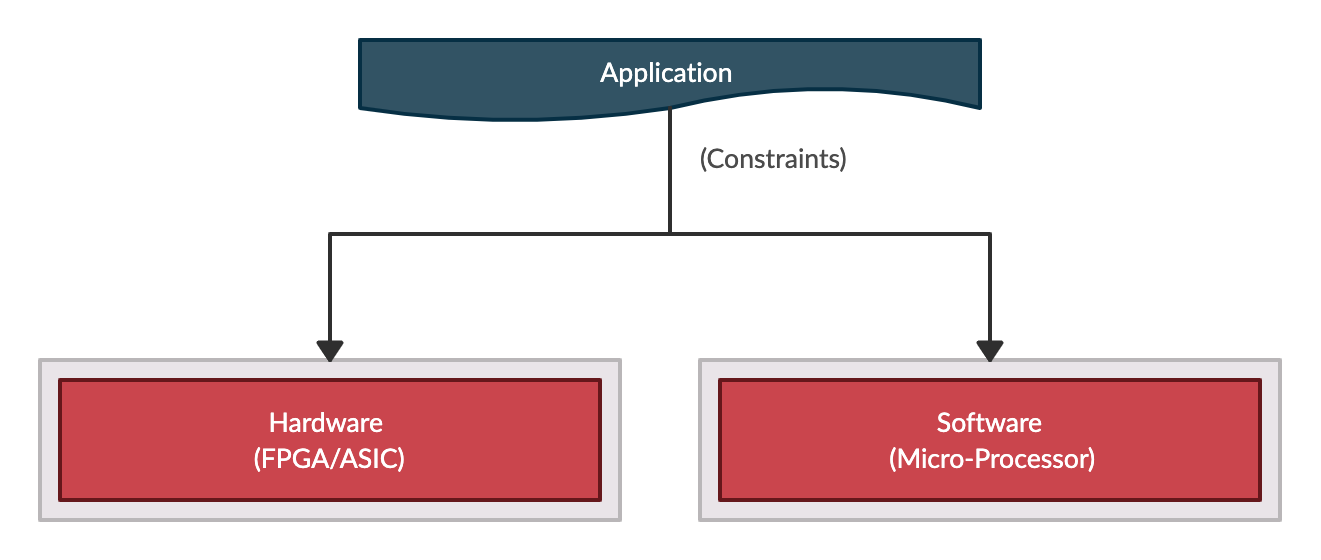
\includegraphics[scale=0.3]{images/problem.png}
%%    \end{center}
%%  \caption{HW/SW Paritioning problem}
%%\end{figure}


\section{Justification for the research}
 
 The debate of state-of-the-art web server architecture is progressing and researchers try to compare the performance of web server architectures by introducing various optimization techniques. In previous researches, new architectures were proposed by fine-tuning existing architectures to increase the overall performance and performance of server have been optimized for different workloads as well. Nevertheless, the performance of server architectures was not compared against different types of programming features especially for various CPU-intensive and IO-intensive applications. In most cases, a uniform workload is used. Moreover, when comparing different server architectures other studies used different frameworks and languages for each architecture.
 
 This research addresses the following areas,
 
 \begin{itemize}
 	\item Implement new server architectures in Ballerina based on popular server architecture models, then performance is compared against different types of programs.
 	\item Identify parameters further to optimize the performance for different types of programming features. 
 	\item A machine learning model is proposed for predicting the optimal parameters ( In this research it is thread pool size) for a given set of programming features.
 \end{itemize}
 
  The initial idea of the research was, providing a clear conclusion on particular server architecture performs well for a given type of program while the performance of another server architecture is better for another type of program by introducing new server architectures and extensive tuning of the implemented server architectures. Based on results gathered in the early stage of this research, the focus was later concentrated on tuning the thread pool size.
 
 None of the previous research has proposed a methodology for the identification of programming features automatically and propose the web server architecture or optimal thread pool size for a given set of programming features. Furthermore, Ballerina is a better candidate for the research because identification of the programming features such as IO operation is more convenient in Ballerina. Features that are difficult to extract in other languages are native to the Ballerina language. 
 

\section{Methodology}

	This research started with implementing new web server architectures in Ballerina and then evaluating the performance of each including the existing architecture (Refer figure \ref{bal_internal}). These architectures are inspired by the Thread per connection model and event-based models(Ex: \acrshort{seda}). This step includes modifying the Ballerina source code. A deeper analysis of existing Ballerina architecture is required to modify the source code for new architectures, otherwise, bugs can affect the performance. 
	
	Performance is evaluated with test programs that consist of different programming features. As an example, one program may consist of several database calls and another program only contain some arithmetic operations. Then performance is evaluated according to program features. The objective is to provide the best performant server architecture for a given Ballerina program with respect to features of that program. Fine-tunes are carried out based on the results of each phase. That led the study to focus on thread pool tuning after several experiments. 
	
	The final model consists of a machine learning model that provides optimal thread pool size for a given program. Figure  \ref{hl_architecture} shows the overview of the research. Steps in the diagram are explained more detail in chapter \ref{chap:3} and section \ref{sec:final_design}.
	
	\begin{comment}
	
		Results are dependent of the deployment environment of the service. Hence, first user need to train the machine learning model with predefined set of programs. The user able to provide own program and the model predict the optimal thread pool size for that program.
	\end{comment}
	
	\begin{figure}[htbp]
		\begin{center}
			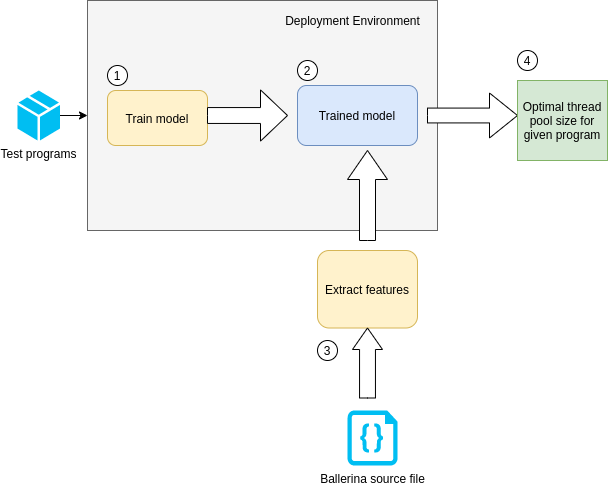
\includegraphics[scale=0.5]{figures/hl_architecture.png}
		\end{center}
		\caption{High-level overview of the research}
		\label{hl_architecture}
	\end{figure}
	

\section{Outline of the Dissertation}

This dissertation outlines 6 chapters as follows.

\begin{enumerate}
	\item Introduction — Contains summarized background study, research problems, justification and overview of the methodology.
	\item Literature Review — Present related studies and theories for this research.
	\item Research Design — Design of the research with respect to each stage of the research.
	\item Implementation — Provide important implication carried out in order to conduct experiments and obtain results. 
	\item Results \& Evaluation — Contain the results obtained in each phase and in depth discussion of the results.
	\item Conclusion — Discuss how the results mentioned in Chapter 5 has addressed the research questions. An emphasis will be given in highlighting the contribution of this research work to the scientific world. Implications of further research will also be discussed in this chapter.
\end{enumerate}

\section{Definitions}

\subsubsection{Concurrency level}

In this research Concurrency level and Concurrent users are used interchangeably referred to as concurrent users who have connected the web server. This value can be simulated in load testing software. A good web server must be able to perform well at a higher concurrency level.

\subsubsection{Deployment environment}

Deployment environment is where web server is deployed and running. Configuration of the environment includes the Operating system, Number of CPU cores, Speed of the CPU, Amount of RAM and Network stability, etc.

\subsubsection{Web Server architecture} \label{sub:def_web_server_architecture}

 Web server architecture provides a clear abstraction of what are the components of web server, how the components are interacting with each other and the behavior of each component when a client request is processed. Thread per connection model \cite{comp_ac} and SEDA \cite{seda} are such two popular server architectures. Thread per connection model spawns a new thread per each client request while SEDA reuses the threads by pooling techniques. New server architectures can be implemented by combining existing models or changing parameters such as the size of the thread pool. Major changes such as adding new components, combining them can be considered as a new architecture while changing parameters such as defining the minimum and the maximum number of threads can be expressed as fine-tuning. Chapter \ref{chap:2} provides in-depth explanation thread pools.

%Results are subjects to the configurations of that environment.

\section{Delimitations of Scope}

\subsection{In-Scope}

\begin{itemize}
	\item Implement new server architectures in Ballerina by modifying the existing implementation. This includes adding and removing new thread pools. Then performance is evaluated using relevant metrics .
	\item Fine tune and optimize the new architectures by identifying bugs and extensive debugging — these tuning includes the changing thread pool size.
	\item Implementing different types of program which have CPU intensive and IO intensive features. Standard ballerina benchmark tools are also referred \cite{Ballerina_Performance}. 
	\item Justification of used tools and accuracy of 
	\item Identify different program features that affect the performance of web sever.
	\item Compare relevant metrics of several machine learning models and hyper parameter tuning of each model in order to get accurate model.
	\item Compare performance of proposed model and current Ballerina sever architecture.  
\end{itemize}

\subsection{Out-Scope}

\begin{itemize}
	\item Generalizing the findings for other languages and frameworks.
	\item Evaluate and compare the results for different deployment environments which have different hardware.
	\item Design and implementation of analytical (a.k.a white box model in this research) model (queuing theory approach etc. ) to predict optimal thread pool size.
\end{itemize}

\section{Conclusion}	

This chapter provides base principles and presents a foundation for the dissertation. In the beginning, the research problem is identified, formulated research questions and research is justified. Then the definitions are presented, the dissertation is outlined, research design and implementation are briefly discussed laying the path to proceed with a detailed explanation of the research.